\documentclass[ignorenonframetext,]{beamer}
\setbeamertemplate{caption}[numbered]
\setbeamertemplate{caption label separator}{: }
\setbeamercolor{caption name}{fg=normal text.fg}
\beamertemplatenavigationsymbolsempty
\usepackage{lmodern}
\usepackage{amssymb,amsmath}
\usepackage{ifxetex,ifluatex}
\usepackage{fixltx2e} % provides \textsubscript
\ifnum 0\ifxetex 1\fi\ifluatex 1\fi=0 % if pdftex
  \usepackage[T1]{fontenc}
  \usepackage[utf8]{inputenc}
\else % if luatex or xelatex
  \ifxetex
    \usepackage{mathspec}
  \else
    \usepackage{fontspec}
  \fi
  \defaultfontfeatures{Ligatures=TeX,Scale=MatchLowercase}
\fi
\usefonttheme{structurebold}
% use upquote if available, for straight quotes in verbatim environments
\IfFileExists{upquote.sty}{\usepackage{upquote}}{}
% use microtype if available
\IfFileExists{microtype.sty}{%
\usepackage{microtype}
\UseMicrotypeSet[protrusion]{basicmath} % disable protrusion for tt fonts
}{}
\newif\ifbibliography
\usepackage{color}
\usepackage{fancyvrb}
\newcommand{\VerbBar}{|}
\newcommand{\VERB}{\Verb[commandchars=\\\{\}]}
\DefineVerbatimEnvironment{Highlighting}{Verbatim}{commandchars=\\\{\}}
% Add ',fontsize=\small' for more characters per line
\usepackage{framed}
\definecolor{shadecolor}{RGB}{248,248,248}
\newenvironment{Shaded}{\begin{snugshade}}{\end{snugshade}}
\newcommand{\KeywordTok}[1]{\textcolor[rgb]{0.13,0.29,0.53}{\textbf{{#1}}}}
\newcommand{\DataTypeTok}[1]{\textcolor[rgb]{0.13,0.29,0.53}{{#1}}}
\newcommand{\DecValTok}[1]{\textcolor[rgb]{0.00,0.00,0.81}{{#1}}}
\newcommand{\BaseNTok}[1]{\textcolor[rgb]{0.00,0.00,0.81}{{#1}}}
\newcommand{\FloatTok}[1]{\textcolor[rgb]{0.00,0.00,0.81}{{#1}}}
\newcommand{\ConstantTok}[1]{\textcolor[rgb]{0.00,0.00,0.00}{{#1}}}
\newcommand{\CharTok}[1]{\textcolor[rgb]{0.31,0.60,0.02}{{#1}}}
\newcommand{\SpecialCharTok}[1]{\textcolor[rgb]{0.00,0.00,0.00}{{#1}}}
\newcommand{\StringTok}[1]{\textcolor[rgb]{0.31,0.60,0.02}{{#1}}}
\newcommand{\VerbatimStringTok}[1]{\textcolor[rgb]{0.31,0.60,0.02}{{#1}}}
\newcommand{\SpecialStringTok}[1]{\textcolor[rgb]{0.31,0.60,0.02}{{#1}}}
\newcommand{\ImportTok}[1]{{#1}}
\newcommand{\CommentTok}[1]{\textcolor[rgb]{0.56,0.35,0.01}{\textit{{#1}}}}
\newcommand{\DocumentationTok}[1]{\textcolor[rgb]{0.56,0.35,0.01}{\textbf{\textit{{#1}}}}}
\newcommand{\AnnotationTok}[1]{\textcolor[rgb]{0.56,0.35,0.01}{\textbf{\textit{{#1}}}}}
\newcommand{\CommentVarTok}[1]{\textcolor[rgb]{0.56,0.35,0.01}{\textbf{\textit{{#1}}}}}
\newcommand{\OtherTok}[1]{\textcolor[rgb]{0.56,0.35,0.01}{{#1}}}
\newcommand{\FunctionTok}[1]{\textcolor[rgb]{0.00,0.00,0.00}{{#1}}}
\newcommand{\VariableTok}[1]{\textcolor[rgb]{0.00,0.00,0.00}{{#1}}}
\newcommand{\ControlFlowTok}[1]{\textcolor[rgb]{0.13,0.29,0.53}{\textbf{{#1}}}}
\newcommand{\OperatorTok}[1]{\textcolor[rgb]{0.81,0.36,0.00}{\textbf{{#1}}}}
\newcommand{\BuiltInTok}[1]{{#1}}
\newcommand{\ExtensionTok}[1]{{#1}}
\newcommand{\PreprocessorTok}[1]{\textcolor[rgb]{0.56,0.35,0.01}{\textit{{#1}}}}
\newcommand{\AttributeTok}[1]{\textcolor[rgb]{0.77,0.63,0.00}{{#1}}}
\newcommand{\RegionMarkerTok}[1]{{#1}}
\newcommand{\InformationTok}[1]{\textcolor[rgb]{0.56,0.35,0.01}{\textbf{\textit{{#1}}}}}
\newcommand{\WarningTok}[1]{\textcolor[rgb]{0.56,0.35,0.01}{\textbf{\textit{{#1}}}}}
\newcommand{\AlertTok}[1]{\textcolor[rgb]{0.94,0.16,0.16}{{#1}}}
\newcommand{\ErrorTok}[1]{\textcolor[rgb]{0.64,0.00,0.00}{\textbf{{#1}}}}
\newcommand{\NormalTok}[1]{{#1}}
\usepackage{graphicx,grffile}
\makeatletter
\def\maxwidth{\ifdim\Gin@nat@width>\linewidth\linewidth\else\Gin@nat@width\fi}
\def\maxheight{\ifdim\Gin@nat@height>\textheight0.8\textheight\else\Gin@nat@height\fi}
\makeatother
% Scale images if necessary, so that they will not overflow the page
% margins by default, and it is still possible to overwrite the defaults
% using explicit options in \includegraphics[width, height, ...]{}
\setkeys{Gin}{width=\maxwidth,height=\maxheight,keepaspectratio}

% Prevent slide breaks in the middle of a paragraph:
\widowpenalties 1 10000
\raggedbottom

\AtBeginPart{
  \let\insertpartnumber\relax
  \let\partname\relax
  \frame{\partpage}
}
\AtBeginSection{
  \ifbibliography
  \else
    \let\insertsectionnumber\relax
    \let\sectionname\relax
    \frame{\sectionpage}
  \fi
}
\AtBeginSubsection{
  \let\insertsubsectionnumber\relax
  \let\subsectionname\relax
  \frame{\subsectionpage}
}

\setlength{\emergencystretch}{3em}  % prevent overfull lines
\providecommand{\tightlist}{%
  \setlength{\itemsep}{0pt}\setlength{\parskip}{0pt}}
\setcounter{secnumdepth}{0}
\definecolor{links}{HTML}{800080}
\hypersetup{colorlinks,linkcolor=,urlcolor=links}

\title{Web Data Collection with R}
\subtitle{HTML Forms GET Case Study}
\author{Peter Meißner / 2016-02-29 -- 2016-03-04 / ECPR WSMT}
\date{}

\begin{document}
\frame{\titlepage}

\begin{frame}
\tableofcontents[hideallsubsections]
\end{frame}

\section{Wikipedia general search}\label{wikipedia-general-search}

\begin{frame}{HTML forms}

\url{http://en.wikipedia.org/w/index.php?title=Special\%3ASearch}

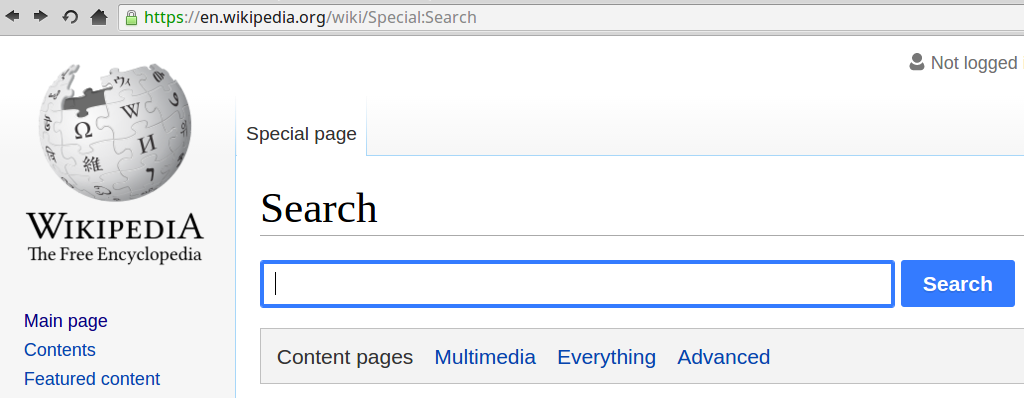
\includegraphics{fig/wikipediasearch.png}

\end{frame}

\begin{frame}[fragile]{inspecting the search bar}

\begin{Shaded}
\begin{Highlighting}[]
\KeywordTok{<form}\OtherTok{ id=}\StringTok{"search"}\OtherTok{ method=}\StringTok{"get"}\OtherTok{ action=}\StringTok{"/w/index.php"}\KeywordTok{>}
  \KeywordTok{<input}\OtherTok{ type=}\StringTok{"hidden"}\OtherTok{ value=}\StringTok{"Special:Search"}\OtherTok{ name=}\StringTok{"title"}\KeywordTok{>}
  \KeywordTok{<input}\OtherTok{ type=}\StringTok{"hidden"}\OtherTok{ value=}\StringTok{"default"}\OtherTok{ name=}\StringTok{"profile"}\KeywordTok{>}
  \KeywordTok{<input}\OtherTok{ id=}\StringTok{"searchText"}\OtherTok{ size=}\StringTok{"50"}\OtherTok{ class=}\StringTok{"mw-ui-input mw-ui-input-inline"}\OtherTok{ type=}\StringTok{"search"}\OtherTok{ value=}\StringTok{"globbel"}\OtherTok{ name=}\StringTok{"search"}\OtherTok{ autocomplete=}\StringTok{"off"}\KeywordTok{>}
  \KeywordTok{<input}\OtherTok{ type=}\StringTok{"hidden"}\OtherTok{ value=}\StringTok{"Search"}\OtherTok{ name=}\StringTok{"fulltext"}\KeywordTok{>}
  \KeywordTok{<input}\OtherTok{ class=}\StringTok{"mw-ui-button mw-ui-progressive"}\OtherTok{ type=}\StringTok{"submit"}\OtherTok{ value=}\StringTok{"Search"}\KeywordTok{>}
\KeywordTok{</form>}
\end{Highlighting}
\end{Shaded}

\url{https://en.wikipedia.org/w/index.php?title=Special\%3ASearch\&profile=default\&search=franken\&fulltext=Search}

\end{frame}

\begin{frame}[fragile]{inspecting the search bar}

\begin{Shaded}
\begin{Highlighting}[]
\KeywordTok{require}\NormalTok{(rvest)}
\NormalTok{url <-}\StringTok{ "http://en.wikipedia.org/w/index.php?title=Special%3ASearch"}
\NormalTok{html <-}\StringTok{ }\KeywordTok{read_html}\NormalTok{(url)}
\end{Highlighting}
\end{Shaded}

\end{frame}

\begin{frame}[fragile]{inspecting the serach bar}

\begin{Shaded}
\begin{Highlighting}[]
\CommentTok{# ADCR: page 236}
\NormalTok{attr_inspector <-}\StringTok{ }\NormalTok{function(parsed_html, xpath)\{}
  \NormalTok{x <-}\StringTok{ }\KeywordTok{html_nodes}\NormalTok{(parsed_html, }\DataTypeTok{xpath=}\NormalTok{xpath)}
  \NormalTok{x <-}\StringTok{ }\KeywordTok{html_attrs}\NormalTok{(x)}
  \NormalTok{x <-}\StringTok{ }\KeywordTok{lapply}\NormalTok{(x, function(x) }\KeywordTok{as.data.frame}\NormalTok{(}\KeywordTok{t}\NormalTok{(x)) )}
  \KeywordTok{do.call}\NormalTok{(plyr::rbind.fill, x)}
\NormalTok{\}}

\KeywordTok{attr_inspector}\NormalTok{(html, }\StringTok{"//form"}\NormalTok{)}
\end{Highlighting}
\end{Shaded}

\begin{verbatim}
##           id method       action
## 1     search    get /w/index.php
## 2 searchform   <NA> /w/index.php
\end{verbatim}

\end{frame}

\begin{frame}[fragile]{inspecting the serach bar}

\begin{Shaded}
\begin{Highlighting}[]
\KeywordTok{attr_inspector}\NormalTok{(html, }\StringTok{"//form[1]//input"}\NormalTok{)[,}\DecValTok{1}\NormalTok{:}\DecValTok{5}\NormalTok{]}
\end{Highlighting}
\end{Shaded}

\begin{verbatim}
##     type          value     name              id size
## 1 hidden Special:Search    title            <NA> <NA>
## 2 hidden        default  profile            <NA> <NA>
## 3 search           <NA>   search      searchText   50
## 4 hidden         Search fulltext            <NA> <NA>
## 5 submit         Search     <NA>            <NA> <NA>
## 6 search           <NA>   search     searchInput <NA>
## 7 hidden Special:Search    title            <NA> <NA>
## 8 submit         Search fulltext mw-searchButton <NA>
## 9 submit             Go       go    searchButton <NA>
\end{verbatim}

\end{frame}

\begin{frame}[fragile]{filling out forms}

\begin{Shaded}
\begin{Highlighting}[]
\KeywordTok{require}\NormalTok{(stringr)}
\NormalTok{url1 <-}\StringTok{ }\KeywordTok{str_c}\NormalTok{(url, }\StringTok{"&search=Peter"}\NormalTok{)}
\NormalTok{url2 <-}\StringTok{ }\KeywordTok{str_c}\NormalTok{(url, }\StringTok{"&search=Peter"}\NormalTok{,}\StringTok{"&fulltext=search"}\NormalTok{)}
\NormalTok{url3 <-}\StringTok{ "http://en.wikipedia.org/w/index.php?search=Peter&fulltext=search"}
\NormalTok{## browseURL(url1)}
\NormalTok{## browseURL(url2)}
\NormalTok{## browseURL(url3)}
\end{Highlighting}
\end{Shaded}

\end{frame}

\begin{frame}[fragile]{filling out forms - more elegant}

\begin{Shaded}
\begin{Highlighting}[]
\KeywordTok{require}\NormalTok{(httr)}
\NormalTok{url  <-}\StringTok{ "http://en.wikipedia.org/w/index.php"}
\NormalTok{resp <-}\StringTok{ }
\StringTok{  }\KeywordTok{GET}\NormalTok{(url, }
      \DataTypeTok{query =} \KeywordTok{list}\NormalTok{(}
        \DataTypeTok{title   =} \StringTok{"Special:Search"}\NormalTok{,}
        \DataTypeTok{profile =} \StringTok{"default"}\NormalTok{,}
        \DataTypeTok{search  =} \StringTok{"Bamberg"}\NormalTok{,}
        \DataTypeTok{fulltext=} \StringTok{"search"}
      \NormalTok{)}
  \NormalTok{)}
\end{Highlighting}
\end{Shaded}

\end{frame}

\begin{frame}[fragile]{filling out forms - more elegant}

\begin{Shaded}
\begin{Highlighting}[]
\NormalTok{xpath =}\StringTok{ "//*[@class='mw-search-result-heading']/a"}
\NormalTok{results <-}\StringTok{ }
\KeywordTok{html_attr}\NormalTok{(}
  \KeywordTok{html_nodes}\NormalTok{(}
    \KeywordTok{content}\NormalTok{(resp, }\StringTok{"parsed"}\NormalTok{), }
    \DataTypeTok{xpath=}\NormalTok{xpath}
  \NormalTok{), }\StringTok{"title"} \NormalTok{)}
\end{Highlighting}
\end{Shaded}

\end{frame}

\end{document}
